\documentclass{article}
\usepackage{graphicx} % Required for inserting images
\usepackage[utf8]{inputenc}
\usepackage{mathrsfs,amsmath}
\usepackage{amssymb}
\usepackage{mathtools}
\usepackage{amsfonts}
\usepackage[parfill]{parskip}
\usepackage{tikz-cd}
\graphicspath{ {./images/} }
\usepackage{biblatex}  %Imports biblatex package
\bibliography{../EE}





\author{Pablo Santos Guerrero}
\date{December 13, 2023}
\title{For which values of $\theta$ is cos$(\theta)$ a constructible number? }

\begin{document}

\maketitle
\begin{center}
\textbf{Word Count} : 3990
\end{center}


\newpage
\tableofcontents
\newpage

\section{Introduction}
 In the study of mathematics, the acquisition of certainty has always been a leading cause for comparison between the natural world and the theoretical one. 
In particular, the study of constructible numbers has been an area of interest since before Christ. The Ancient Greeks had a keen interest in plane geometry by strictly using only circle constructions and indefinitely long line segments.
The concept of constructibility was coined by the Greeks when immersed in the discussion of impossible geometric expressions of numbers since it implied that there was a limit to which numbers could be drawn by a compass and straight edge.
\par
The focus of this essay is to explore the values for which the cosine of angles are constructible by using Field Theory and Galois Theory, developed in the 18th 
and  19th century. The process of reaching a set of values for $\theta$ for which cos$(\theta)$ is a constructible number requires findings gathered from different mathematicians in history and it has become a well-known topic because of the elegance of the problem's unraveling. 
\par
First, we must introduce the concept of constructability and the way in which mathematicians study constructions algebraically. It is essential to familiarize ourselves with Galois Theory to be able to justify the solvability of polynomials and specifically the algebraic structure of cyclotomic polynomials; they create regular $n$-sided polygons with roots corresponding to vertices in an Argand Diagram. Finally, the goal is to find a sufficient set for $n\in\mathbb{Z}$ such that cos($\frac{2\pi}{n}$) is constructible.

\section{Constructions}
\par 
\subsection{Euclidean Axioms}
We begin by stating the 3 Euclidean axioms which define what a Euclidean construction is. It is, a finite number of operations of the following type:
    \begin{itemize}
        \item[\textbf{(1)}] Given two points, draw a line from one to the other with arbitrary distance.
        \item [\textbf{(2)}] Create a continuous straight line with finite length.
        \item[\textbf{(3)}] Produce a circle with any point as a center and radius of arbitrary length.
    \end{itemize}
\par
Given a unit length, it is simple to begin extending numbers and combining these operations to create specific shapes and arbitrary lengths with geometric properties. For example, constructions of the perpendicular bisector of a line and angle bisection using \textbf{(1),(2),(3)}.
\par
\subsection{Operations}
A number is \textit{constructible} if its length can be constructed through a finite number of Euclidean Constructions.
\par
Compass and straightedge have 6 fundamental operations that we must consider to operate with all the numbers which can be expressed by a finite number of Euclidean constructions. For example, given a unit length, one can add and find the difference between two line segments by projecting one next to the other or by projecting it on top of it, respectively. On the other hand, to find the product and division of 2 numbers, the following triangle constructions are used based on the ratios between the lengths. 
%Diagram 1
\begin{figure}[ht]
\caption{Product of Constructible Numbers $^{\textrm{\footnotesize\cite{geoMult}}}$}
\centering
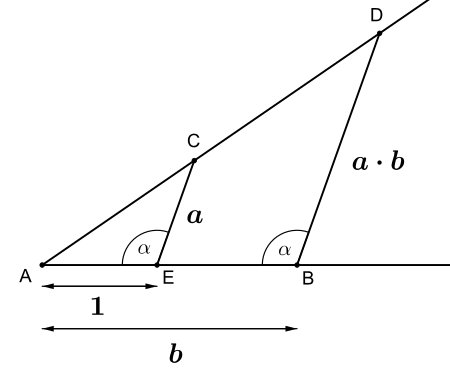
\includegraphics[width=0.5\textwidth]{../images/Constructible_multilply.png}
\end{figure}
%DIAGRAM2
\begin{figure}[ht]
\caption{Quotient of Constructible Numbers $^{\textrm{\footnotesize\cite{geoDiv}}}$}
\centering
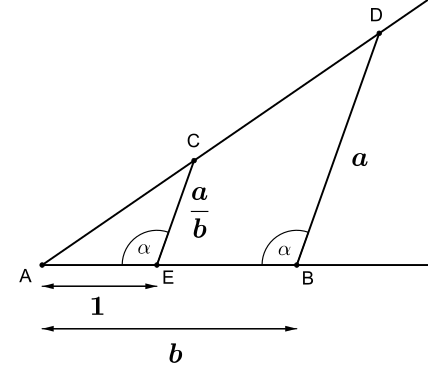
\includegraphics[width=0.5\textwidth]{../images/Constructible_div.png}
\end{figure}


\section{Field Theory}
\subsection{Polynomials}
 Modern algebraists have gathered an enormous amount of research with regard to the phenomenal findings of a young mathematician called Évariste Galois.  At a young age, he substantiated sufficient conditions in a given polynomial to express the solubility by radicals of that polynomial, by specifically looking at the permutations of roots called the Galois group of a polynomial. In his writings, Galois had the ambition to find the accepted conditions for a polynomial to be reducible into linear factors and became one of the most influential inputs into polynomial understanding. 

\par
\paragraph{Definition:} A Ring of polynomials refers to a specific type of polynomials where the coefficients $a_i$ are elements of a unique set, this way we may classify polynomials by their coefficients. For example:

$$\mathbb{Q}\lbrack x\rbrack=\lbrace \sum_{i=0}^{n}a_{i}x^{i} \mid a_i\in\mathbb{Q}\rbrace$$



\subsection{Algebraic Constructions}
Since constructions are drawn in  2-dimensional planes, they are considered using a \textit{real vector space} $\mathbb{R}^{2}$. Specifically, mathematicians use complex numbers to interpret the vector plane since there is a bijection that corresponds $\mathbb{R}^{2}$ to $\mathbb{C}$. Doing so, one can emulate addition, multiplication, and their inverses in $\mathbb{C}$ without division by $0$.

\par
It is important to define the Groups and Fields because of their relevant properties.
\paragraph{Definition:} 
A group is an ordered pair $(G,\ast)$ where $G$ is a set and $\ast$ is a binary operation on $G$ satisfying the following axioms:

\begin{itemize}
    \item[\textbf{(1)}] $(a \ast b) \ast c = a \ast (b \ast c)$ for all $a, b, c \in G$. The operation $\ast$ is \textit{associative}.
    \item[\textbf{(2)}] There exists an element $e \in G$ called the \textit{identity} such that for all $a \in G$, $a \ast e = a$.
    \item[\textbf{(3)}] The number of elements in the group is the \textit{order} denoted $\mid G \mid = n, n\in\mathbb{Z}^{+}$
\end{itemize}

\paragraph{Definition $^{\textrm{\footnotesize\cite{DummitFoote}}}$:}  Let $G,N$ be groups such that $N\subseteq G$, and $n\in N, g \in G$, then $gng^{-1}$ is called the conjugate of $n$ by $g$. The set $gNg^{-1} = \lbrace gng^-1, n\in N \rbrace$ is called the conjugate of $N$ by $g$. The element $g$ is said to 
\textit{normalize} $N$ if $gNg^{-1} = N$. Subgroup $N$ is called $normal$ if every element of $G$ normalizes it. If $N$ is a normal subgroup of $G$ then write $N \trianglelefteq G$.


\paragraph{Definition $^{\textrm{\footnotesize\cite{SheldonAxler}}}$:} A vector space is a set $V$ along with an addition on $V$ and a scalar multiplication on $V$ such that the following properties hold for all, $u,v,w\in V$:
    \begin{itemize}
        \item[\textbf{Commutativity}]: $u + v = v + u$
        \item[\textbf{Associativity}]: Like in a group.
        \item[\textbf{Additive Identity}]: There exists an element $0 \in V$ such that $v + 0 = v$
        \item[\textbf{Additive Inverse}]: For every $v \in V$ there exists a $w \in V$ such that $v + w = 0$
        \item[\textbf{Multiplicative Identity}]: There exists a $1\in V$ such that $1v = v$
        \item[\textbf{Distributive Properties}]: $a(v + w) = av + aw$ and  $(a + b)v = av +bv, \forall a,b \in \mathbb{C}$
        
    \end{itemize}

\paragraph{Definition $^{\textrm{\footnotesize\cite{SheldonAxler}}}$:} A linear combination of a list $v_1,...,v_m$ of vectors in $V$ is a vector of form:

$$ a_1v_1 + ... +a_m v_m$$

\paragraph{Example:} The vector $\vec{a} = (8 , 18)$ is a linear combination of vectors $\vec{q} = (2, 4)$ and $\vec{r} = (1, 3)$ all elements of $\mathbb{R}^2$ because

$$\vec{a}= 3\vec{q} + 2\vec{r} = 3(2, 4) + 2(1, 3) = (6 + 2, 12 + 6) = (8, 18).$$

\paragraph{Definition $^{\textrm{\footnotesize\cite{SheldonAxler}}}$:} The set of all linear combinations of a list of vectors $v_1,...,v_m\in V$ is called the \textit{span} of $v_1,...,v_m$, denoted $\text{span}(v_1,...,v_m)$. The span of the empty list () is $\lbrace 0 \rbrace$. If $ V = \text{span}(v_1,...,v_m) = V$ we say that $v_1,...,v_m$ spans $V$.


\paragraph{Definition $^{\textrm{\footnotesize\cite{SheldonAxler}}}$:} A \textit{basis} of $V$ is a list of vectors in $V$ that is linearly independent and spans $V$.

\par
A field is a vector space that has 2  distinct operations with multiplicative inverse between elements without $0$. Applying any of the operations to any of the elements of the field will lead to another element. Since constructible numbers can be added and multiplied, the inverses can be applied respectively by subtraction and division. Hence, Constructible numbers create a field $F = \mathbb{Q}$ under the addition and multiplication operations. 

\par
Additionally, one can construct the square root of a constructible number by using the geometric mean within a circle. This operation allows the extension of the field $\mathbb{Q}$ since all rationals can be square-rooted indefinitely. This is known as an Euclidean Field $\mathbb{K}$, which includes all extensions that can be created using the operation or construction from Figure 3. Any constructible number belongs to the Euclidean Field.


%DIAGRAM 3
\begin{figure}[ht]
\caption{Square root of Constructible Number $^{\textrm{\footnotesize\cite{geoMean}}}$}
\centering
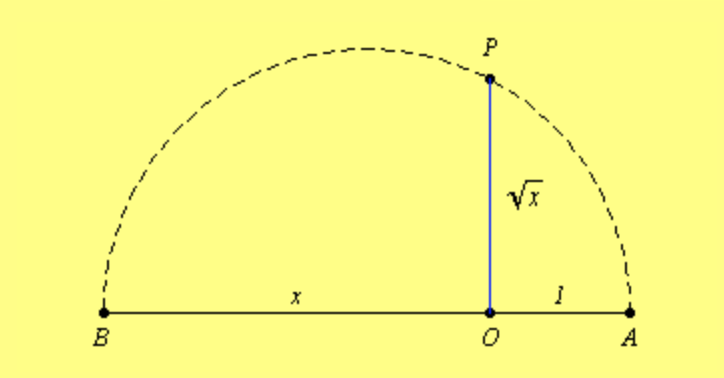
\includegraphics[width=0.5\textwidth]{../images/Screen Shot 2023-10-05 at 1.01.06.png}
\end{figure}
\paragraph{Example:}
The number $k=\sqrt{2}$ is constructible because 2 is constructible, however since $k\notin\mathbb{Q}$ it can be found in the smallest field $L\subset \mathbb{C}$ such that:
 
$$ L = \lbrace a + b\sqrt{2} ; a,b \in\mathbb{Q} \rbrace$$

Elements of $L$ include:
$$l = 3 + 4\sqrt{2}$$
$$w = -3\sqrt{2}$$
$$ l + w = (3 + 4\sqrt{2}) + (-3\sqrt{2}) = 3 + (4-3)\sqrt{2} = 3 + \sqrt{2} $$
$$lw = (3 + 4\sqrt{2})(-3\sqrt{2}) = -9\sqrt{2} -12(2) = -24 - 9\sqrt{2}. $$

We denote $L = \mathbb{Q}(k) = \mathbb{Q}(\sqrt{2})$ as an extension of the rationals. This is known as a \textit{field extension}. It is an inclusion relationship between $\mathbb{Q}$ and $\mathbb{Q}(\sqrt{k})$ with a function $\psi$ such that:

$$\psi:\mathbb{Q}\mapsto\mathbb{Q}(\sqrt{k}) \quad $$

\subsection{Field Extensions}
\par
We say a polynomial is solvable by radicals if it can be written as a product of linear factors by manipulating the coefficients using the additive, multiplicative, and radical operations. This is \textit{splitting} the polynomial into the form:

$$p(x) = \prod_{i=0}^{n}(x-\alpha_{i}), \alpha_i\in L \subseteq \mathbb{C}$$

Were $\alpha_i$ are the roots of $p$. We say $p(x)$ is \textit{reducible} if $L$ is the smallest field that satisfies this for $p(x)$; if not then it is \textit{irreducible}. 

\paragraph{Example:} The polynomials $p(x)$ and $h(x)$ are reducible since
$$p(x) = x^2-1 = (x+1)(x-1); \pm 1\in \mathbb{Q}\subseteq\mathbb{C}$$
$$h(x) = x^4 +x^2 - 6 = (x+i\sqrt{3})(x-i\sqrt{3})(x+\sqrt{2})(x-\sqrt{2}); \pm i\sqrt{3},\pm\sqrt{2}\in L \subseteq \mathbb{C}$$

\paragraph{Definition $^{\textrm{\footnotesize\cite{DummitFoote}}}$:} If $L$ is a field containing the sub-field $L_{0}$, then $L$ is said to be a \textit{field extension} of $L_0$ denoted $L:L_{0}$ or by diagram:


$$\begin{tikzcd}[row sep=large, column sep=large]
    L \arrow[dash]{d} \\
    L_0
\end{tikzcd}$$

In general, let $L_0 = \mathbb{Q}$ and $L_1 = \mathbb{Q}(\alpha_1)$, then any \textit{constructible} number $k$ must be an element of a field 
$$L_n = \mathbb{Q}(\alpha_1, \alpha_2, ... , \alpha_n) = \lbrace p\alpha_1 + q\alpha_2 + ... + s\alpha_n ; p,q,s\in\mathbb{Q} \rbrace$$

created by a finite number of extensions from the base field $L_0$. Visually:

$$\begin{tikzcd}[row sep=small, column sep=tiny]
    & L_n \arrow[dash]{dd} \\
    & \\
    & ... \arrow[dash]{dd} \\
    & \\
    & L_{1} \arrow[dash]{dd} \\
    & \\
    & L_0  \\
    & \\
\end{tikzcd}$$


\subsection{Degree of an Extension}
The map $\psi$ defines a dimension over its base field, specifically a vector space. This is known as the \textit{degree of an extension}. Using the vector space, we can find multiplicative properties in degrees of extension to simplify and deconstruct field extensions. To do so, we must use linear independence.

\paragraph{Definition $^{\textrm{\footnotesize\cite{SheldonAxler}}}$:} A vector space is called \textbf{finite-dimensional} if some list of vectors in it spans the space.

\paragraph{Definition $^{\textrm{\footnotesize\cite{TomLeinster}}}$:} The \textbf{degree} $[L: \mathbb{Q}]$ of a field extension $L : \mathbb{Q}$ is the dimension of $L$ as a vector space over $\mathbb{Q}$.
\par
To find the degree, one must use the monomial of the smallest power of $x$ with the number $\alpha$ as a root. This is the \textit{minimal polynomial} $m$ of the extension to the field containing $\alpha$. The degree $\partial m$ of the extension $\lbrack \mathbb{Q}(\alpha) : \mathbb{Q} \rbrack$ is the number of distinct solutions of the minimal polynomial of $\alpha$ :

$$\lbrack \mathbb{Q}(\alpha) : \mathbb{Q} \rbrack = d = \partial m , d\in\mathbb{Z}^{+}$$

\paragraph{Example:}
The extension $\mathbb{C}:\mathbb{R}$ has a degree of 2 because $\mathbb{C} = \mathbb{R}(i)$. The dimension of $\mathbb{C}$ over $\mathbb{R}$ is 2 and the minimal polynomial of $i = \alpha$ is $f(x) = x^2 + 1$ with degree of 2. This leads to a useful property of field extensions known as the Tower Law.

\paragraph{Theorem (Tower Law) $^{\textrm{\footnotesize\cite{GaloisStewart}}}$:} If $L : F$ has $[ L : F ] = n, n\in\mathbb{Z}^{+}$ and $M$ is a field such that $ F \subseteq M \subseteq L$, then 
$ [ L : F ] = [ L : M ][ M : F ] = n $.
\par
\textit{Proof} $^{\textrm{\footnotesize\cite{Milne}}}$: 
\par
If $L$ is finite over $F$, then it is certainly finite over $M$; moreover, $M$, being a
subspace of a finite-dimensional $F$-vector space is also finite-dimensional.
\par Thus, assume that $L:M$ and $M:F$ are of finite degree and let $(m_i)$ for $1\leq i \leq k$ be a basis for $M$ as a vector space over $F$ and let $(l_j)$ be a basis for $L$ as a vector space over $M$ for $1\leq j \leq r$.
First, $(m_i l_j)_{i,j}$ spans $L$. Let $\omega \in L$. Then, because $(l_j)_j$ spans $L$ as vector space over $E$,
$$\omega = \Sigma_j \kappa_j l_j$$
for some $\kappa_j\in M$. Since $(m_i)_i$ spans $M$ as a vector space over F,

$$\kappa_j = \Sigma_i a_{ij} m_i.$$

And by putting them together we have:
$$\omega = \Sigma_j \Sigma_i a_{ij} m_i l_j.$$

Second, we know $(m_i l_j)_{i,j}$ is linearly independent. A linear relation $\Sigma a_{ij} m_i l_j = 0 \quad a_{ij}\in F$, can be written as $\Sigma_j (\Sigma_i a_{ij} m_i) l_j = 0$. The linear independence of the $l_j$  shows that $\kappa_j = \Sigma_i a_{ij} m_i = 0$ for each $j$, and the linear independence of the $m_i$ show that $a_ij = 0$. $\Box$

\paragraph{Outline of Proof:}
The proof uses the basis of each field extension and tests the effect of multiplying the linearly independent vector lists to see if the result is another basis. By first defining the basis of each extension, because of linear independence, the sum of the span must be equal to zero. Thus we can find a suitable expression for the linear combination $\omega$ element of $L$ and an expression for each $\alpha_j$ element of $M$. As we can see, the effect of substituting one into the other is another linear combination element of the basis $(m_i l_j)_{i,j}$, hence $L: F$ is a finite-dimensional vector space. We can therefore name 2 properties for field extensions:


\paragraph{Definition:} A field extension $L_n:L_0$ - were $L_n$ is the smallest field containing $\alpha$ - is called \textit{algebraic} over $L_0$ if there exists a \textit{finite} sequence of field extensions:

$$L_0 \subseteq L_1 \subseteq ... L_{n-1} \subseteq L_n \subseteq \mathbb{C} $$

From the Tower Law, it follows immediately that $ [ L_n : L_0 ] = n$ for some $n\in\mathbb{Z}^{+}$. $L_n:L_0$ is an \textit{finite extension}.

\par
If an extension is not finite it is \textit{trascendental}.
\par
Recall that the Euclidean Domain is bounded by square roots, which means that if a constructible number $k$ is an element of $\mathbb{Q} = L_0$ then $\sqrt{k}\in L_1$ where $[ L_1: L_0 ] = 2$ since the minimal polynomial of $\sqrt{k}$ is a quadratic equation at most.

\subsection{Normality}
\paragraph{Definition $^{\textrm{\footnotesize\cite{GaloisStewart}}}$:} A sub-field of $\mathbb{C}$ is the splitting field for a nonzero polynomial $f\in L_0$ if $L_0\subseteq T$ for any field $T$ such that:
\begin{itemize}
    \item[\textbf{(1)}] $f$ splits over $T$.
    \item[\textbf{(2)}] $T=L_0(\alpha_1,\alpha_2, ... ,\alpha_n)$ and $f(\alpha_j)=0, j=1,2,...,n.$
\end{itemize}
\par
For notation purposes, the splitting field of $f$ over a base field $L_0$ is split$_f(L_0)$. For constructible numbers, we know then that if a number is constructible it follows immediately that there exists a splitting field which contains it. To be able to find the extension to any algebraic number, it is necessary to define one last property of these extensions.

\paragraph{Definition $^{\textrm{\footnotesize\cite{GaloisStewart}}}$:} An algebraic field extension $L_n : L_0$ is \textit{normal} if every irreducible polynomial over $L_0$ that has at least one zero in $L_n$ splits.

\paragraph{Example:} The polynomial $f(x)=x^3-5$ does not split in $\mathbb{Q}$. If we extend the field to $\mathbb{Q}(\sqrt[3]{5})$, we know $\alpha=\sqrt[3]{5}$ is a root of $f$ and thus there is at least one zero in the field. However, since $f$ has complex roots it doesn't split fully and hence is not normal by definition.
 We reach a crucial theorem that relates the normality of polynomials to the splitting field of its roots.

 \paragraph{Theorem $^{\textrm{\footnotesize\cite{GaloisStewart}}}$:} A field extension $L: K$ is \textit{normal} and \textit{finite} if and only if $L$ is the splitting field for any $P\in K[x]$.
 \par
\textit{Proof} $^{\textrm{\footnotesize\cite{GaloisStewart}}}$:
\par
Suppose $L:K$ is normal, then we know $L = K(\alpha_1,\alpha_2, ... ,\alpha_n)$ for all $\alpha_i$ algebraic  over $K$ and $1 \leq i \leq n$.  Let $m_j$ be the minimal polynomial of $\alpha_i$ over $K$ and $f=\prod_{i}m_i$. Each $m_j$ is irreducible over $K$ and has zero $\alpha_i\in L$ so by normality, each $m_j$ splits over its base field $K$. Hence $f$ splits over $L$ because $ L = K(\alpha_1,...\alpha_n)$.
\par 
To prove the converse suppose that $L$ is the splitting field to some polynomial $g\in L[x]$, then $L$ is finite. To find normality let $f\in L[x]$ be a polynomial irreducible over $K$ with a zero in $L$. Additionally, let $M\supseteq L$ be the splitting field of $fg$ over $K$, suppose $\phi_{1,2}$ are zeros of $f$ in $M$. By irreducibility, $f$ is the minimal polynomial of $\phi_{1,2}$ over $K$. The claim is that $[L(\phi_1): L]=[L(\phi_2): L]$. We deconstruct the tower of sub-fields of $M$ as two corresponding chains for $\phi_j,j=1,2$:
$$K\subseteq K(\phi_j) \subseteq L(\phi_j) \subseteq M,$$ by the tower law the degree of the extension $M:K$ is,

$$[L(\phi_i): L][L:K] = [L(\phi_i): K] = [L(\phi_i): K(\phi_i)] [K(\phi_i): K].$$ 

Since $\phi_{1,2}$ have same minimal polynomial over $K$,
$$[K(\phi_1): K][L:K] = [K(\phi_2): K]$$

and thus $L(\phi_j)$ is splitting field of $g$ over $K(\phi_j)$. The extensions $K(\phi_2)$ and $K(\phi_2)$ are then isomorphic. By substituting the $j$'s:

$$[L(\phi_1): K(\phi_1)] [K(\phi_1): K] =  [L(\phi_2): K(\phi_i)] [K(\phi_2): K]$$
$$ [L(\phi_1): L][L:K] = [L(\phi_2): L][L:K]$$
$$[L(\phi_1): L] = [L(\phi_2): L]$$ as claimed. Hence $L:K$ is normal. $\quad \Box$ 
\par
Finally, to find the splitting field of constructible numbers, the extensions must be normal and finite. We can turn to constructibility in terms of field theory.

\subsection{Constructible Number Theorem}
For any constructible $k\in\mathbb{C}$ and let $L_n$ be its splitting field over $\mathbb{Q} = L_0$, we know $k\in\mathbb{K}$ and $\mathbb{K}$ is bounded by all finite quadratic extensions such that:

$$[L_n : L_0] = [L_n : L_n-1] [L_n-1 : L_n-2] ...[L_1 : L_0] [L_0 : L_0] $$
$$[L_n : L_0] = 2\times 2...\times2\times 1 = 2^j,j\in\mathbb{Q}.$$

\paragraph{Theorem:} Any $k\in\mathbb{C}$ is constructible if and only if there exists an irreducible polynomial $p\in L_0[x]$ and a $j\in\mathbb{Z}^{+}$ where:

$$\partial p = 2^j \quad \textrm{and} \quad p(k) = 0.$$

\textit{Proof}$^{\textrm{\footnotesize\cite{ConstructibleNumberT}}}$:
\par By induction, 
\par
 base: let $L_0 = \mathbb{Q}$, and let $k\in\mathbb{Q}$. The minimal polynomial of $k$ is $g(x) = x-k$ because $g(k) = k-k = 0$ and thus root is $x_0 = k$. Since $x_1\in\mathbb{Q}$ then $\partial g = 2^0$.
\par
Inductive step: Assume that for $k\in L_i$, there exists a $p\in\mathbb{Q}[x]$ such that $\partial p = 2^m$ and $p(k) = 0, x_i = k$ holds, this means $[L_{i}: L_0] = 2^m$ .
\par
Let $\zeta\in L_{i+1},g(\zeta) = 0$ then if $\zeta\in L_i$, $\zeta$ and $x_i = k$ have the same minimal polynomial over $\mathbb{Q}$. Additionally, we know that $[L_{i+1}: L_i] = 2^0 = 1$.
\par 
However, if $\zeta\notin L_i$ then $[L_{i+1}: L_i] = 2$ since extension must have minimal polynomial $h(k) = 0, \partial p = 2$ over $L_i$. We can compute that the extension $L_{i+1} : L_0$ has a degree of:

$$ [L_{i+1}: L_0] =[L_{i+1}: L_i][L_{i}: L_0] = 2 \times 2^m = 2^{m+1} = 2^j,j\in\mathbb{Z}^{+},$$

and by definition the minimal polynomial of $k$ has $\partial p = 2^j$ where $p(k) = 0$ and $k\in L_{i+1}. \quad \Box$

\paragraph{Outline of Proof:}
The proof is done by induction (\textit{Salomone}, 2014) to demonstrate how each extension has a degree with a power of 2 and that each constructible number has a splitting field over the rationals. The first step is trivial since the degree of the extension is one and $2^0 = 1$. For the inductive step, we assume that for the $i$-th step, there is a polynomial with solution in the respective field with the degree of polynomial being a product of 2 and degree of extension as well. The proof proceeds to show how the $ i+1$ step also has a reducible polynomial and a finite degree of field extension. If the $i$-th step implies $i+1$ and the base field is true, then the proof is complete. 

\par

Now we know the conditions required so any $z\in\mathbb{K}\subset\mathbb{C}$ is constructible. Explicitly we can look for the constructibility of $z = \text{cos}(\frac{2\pi}{n})$ . If $p(z) = 0$ for $p\in\mathbb{Q}[x]$,  by normality of the extension $\mathbb{Q}(z) : \mathbb{Q}$, $p$ must split in the smallest field containing $z$ and  $[\mathbb{Q}(z) : \mathbb{Q}] = 2^j$.

\par
To find a polynomial, since $z\in\mathbb{C}$, express it in terms of its real and imaginary parts. From Euler's Formula, it is possible to extract the exact value of $z$:

$$\text{cos}(\frac{2\pi}{n}) + i\text{sin}(\frac{2\pi}{n}) = e^{i{\frac{2\pi}{n}}}$$
$$cos(\frac{2\pi}{n}) = \Re(\text{cos}(\frac{2\pi}{n}) + i\text{sin}(\frac{2\pi}{n})) = \Re(e^{i{\frac{2\pi}{n}}})$$ 

for any $\gamma_n = e^{i{\frac{2\pi}{n}}}$, and so if $\gamma_n$ is constructible,  so is its real part and $$[\mathbb{Q}(e^{i{\frac{2\pi}{n}}}) : \mathbb{Q}] = 2^j,j\in\mathbb{Z}^{+}.$$

The numbers complex numbers with the form $$\gamma_{n}^{t} = e^{i{\frac{2t\pi}{n}}}$$ where $\text{gcd}(n, t) = 1$ are known as the primitive nth roots of unity. $^{\textrm{\footnotesize\cite{WikipediaRoots}}}$ Particularly, they are the distinct roots of the polynomial with form:

$$\Phi_n(x)  = \prod_{k = 1}^{\varphi(n)} (x- \gamma_k).$$

This is the cyclotomic polynomial, and it is related to the polynomial $x^n-1$ in the form:

$$x^n-1 = \prod_{d \vert n} \Phi_d(x). \quad ^{\textrm{\footnotesize\cite{WikipediaRoots}}}$$







Since all primitive roots  are powers of $\gamma_n$, the splitting field of $\Phi_n(x)$ is $\mathbb{Q}(\gamma_n)$ since $\gamma_{n}^{t}\in\mathbb{Q}(\gamma_n)$. Additionally, we know that the number of solutions of $\Phi_n(x)$ is $\varphi(n)$ which refers to "the number of integers $t$ in the range $1 \leq t \leq n$ for which the greatest common divisor gcd(n, t) is equal to 1" $^{\textrm{\footnotesize\cite{WikipediaG}}}$. The focus of the essay becomes to prove for which $n$ does $\Phi_n(x)$ and $\gamma_n$ satisfy properties for constructible numbers:

\begin{itemize}
        \item[\textbf{(Condition 1)}] Finite Tower of field extensions to the splitting field. 
        \item [\textbf{(Condition 2)}] $[\mathbb{Q}(\gamma_n):\mathbb{Q}] = 2^j$.
    \end{itemize}

\section{Galois Theory}
To find \textbf{condition 1}, we must demonstrate that $\gamma_n$ is expressible as a finite number of quadratic extensions. Galois proved the existence of a bijection between the sub-fields of the splitting field of a polynomial and the normal subgroups of the group of permutations that preserve relations within the roots: the Galois group.

\subsection{Galois Groups}
\par
Let $K\subseteq L \subset\mathbb{Q}$, $p\in\mathbb{Q}[x]$ and $L:K$ be a finite normal extension and $p$. Consider a function $\sigma$ for all $x,y \in L$ and $k\in K$ with the following properties:
$$\sigma : L \mapsto L$$
    \begin{itemize}
        \item[(1)] $\sigma(x*y) = \sigma(x) * \sigma(y).$
        \item [(2)] $\sigma(k) = k$ (conjugacy).
        \item[(3)] $\sigma$ is bijective.
    \end{itemize}
\par
All functions $\sigma$ are called $K$-automorphisms of $L$ (denoted Aut($L/K$)) and they permute the roots $\alpha_i$ of $p$, the effect of $\sigma$ on $p$ is the following:

$$\sigma(p(x))=\sigma(\sum_{i=0}^{n}a_{i}x^{i})$$
$$\sigma(p(\alpha))= \sigma(0) = \sigma(\sum_{i=0}^{n}a_{i}\alpha^{i})$$ 
Using (1), $\sigma(a_{i}\alpha^{i}) = \sigma(a_i)\sigma(\alpha^i)$. Using (2), since $p(x)\in\mathbb{Q}[x]$ $\sigma(a_i) = a_i$, thus:

$$ \sigma(0) = \sigma(\alpha - \alpha) = \sum_{i=0}^{n}a_{i}\sigma(\alpha)^{i} $$
$$ \sigma(\alpha) - \sigma(\alpha) = \sum_{i=0}^{n}a_{i}\sigma(\alpha)^{i} $$
$$0 = \sum_{i=0}^{n}a_{i}\sigma(\alpha)^{i} $$

The effect of $\sigma$ is clear because we know that $\sigma(\alpha) \ne \alpha$, however  $\sigma(p(\alpha)) = p(\sigma(\alpha)) = 0$. And so the  Aut($L: K$) preserves this relation.

\paragraph{Theorem $^{\textrm{\footnotesize\cite{GaloisStewart}}}$:}If $L:K$ is a field extension, then the set of Aut($L:K$) forms a group under composition of maps:
\par
\textit{proof} $^{\textrm{\footnotesize\cite{GaloisStewart}}}$:
\par 
Suppose  $\alpha$,$\beta$ are Aut($L:K$). Then $\alpha\beta$ is as well since it is an automorphism and $\alpha\beta(k)=\alpha(k) = k, \forall k\in K$. The identity map on $L$ is obviously an Aut($L: K$). and so is $\alpha^{-1}$ because for $K\in K$ we have 
$$k = \alpha^{-1}\alpha(k) = \alpha^{-1}(k)$$
The composition of maps is associative and thus the set of Aut($L: K$) is a group. $\Box$

\paragraph{Definition $^{\textrm{\footnotesize\cite{GaloisStewart}}}$:} The \textit{Galois Group} $\Gamma(L:K)$ of a field extension $L:K$ is the group of all Aut($L:K$) under the operation of composition of maps.

\paragraph{Definition $^{\textrm{\footnotesize\cite{Artin}}}$:} A group is said to be \textit{solvable} if it contains a sequence of $G = G_1 \supseteq G_2 \supseteq ... \supseteq G_n = 1$, each a normal subgroup of the preceding and with $G_{i-1}/G_i$, the quotient group is Abelian/commutative.

\paragraph{Example}: let $p(x) = x^4 + ax^2 + b \in \mathbb{Q}[x]$ by Sridharacharya's rule:
$$\textrm{if} \quad \rho = \frac{a}{2} \quad x^2 = -\rho \pm \sqrt{\rho^2-b}$$
$$x_{1,2} = \pm \sqrt{-\rho + \sqrt{\rho^2-b}}$$
$$x_{3,4} = \pm \sqrt{-\rho - \sqrt{\rho^2-b}}$$

The approach that follows was taken from YouTube video Galois Theory II by (NJ Wildberger)$^{\textrm{\footnotesize\cite{Wildberger}}}$. It resembles Lagrange's method of resolvents which consisted of studying relations based on algebraic properties between roots when permuted, this allowed further interpretation of the structure of the Galois group.
\par
With the above expressions, it is possible to create two relationships over the basis of $\mathbb{Q}$:
$$R_1 : x_1 +x_2 = 0$$
$$R_2 : x_3 +x_4 = 0$$
The group of permutations (written in cyclic notation) which preserve this relationship is:

$$ G_1 = \lbrace e \quad (12) \quad (34) \quad (12)(34) \quad (24)(31) \quad (23)(41) \quad (1324) \quad (1423) \rbrace$$
Now, we extend the basis of the field to $\mathbb{Q}(\eta)$ by using the substitution $\eta = \sqrt{\rho^2 -b}$ and create new relation:
$$R_3 : x_2^2-x_3^2=\eta \quad \textrm{for}$$
$$x_{1,2} = \pm \sqrt{-\rho + \eta}$$
$$x_{3,4} = \pm \sqrt{-\rho - \eta}$$

The new group of permutations which preserves $R_3$ is

$$G_2 = \lbrace e \quad (12) \quad (34) \quad (12)(34) \rbrace.$$

Sequentially we can create 2 final relations; create 2 similar substitutions : $\mu = \sqrt{-\rho + \eta}$ and $\delta = \sqrt{-\rho - \eta}$, in fact they are conjugates under $\eta$. For $\mu$ the relation is

$$R_4 : x_3 - x_4 = 2\mu \quad \textrm{and its group of permutations is} \quad G_3 = \lbrace e \quad (12) \rbrace$$

with basis over $\mathbb{Q}(\eta,\mu)$. Finally the last relation is trivial because $\delta = \sqrt{-\rho - \eta}$ and the relationship

$$ R_5 : x_1 - x_2 =2\delta \quad \textrm{has group of permutations} \quad G_4 = \lbrace e \rbrace$$

the roots of $p(x)$ are:

$$x_{1,2} = \pm \delta$$
$$x_{3,4} = \pm \mu$$

It is clear that there is a finite sequence of groups. The group of permutations generated at each field extension expresses conjugacy over its base field and is hence a Galois group. since $G_1 = \Gamma(\mathbb{Q}(\eta,\mu,\delta) : \mathbb{Q})$, which fixed all elements of $\mathbb{Q}$. $G_2 = \Gamma(\mathbb{Q}(\eta,\mu,\delta) : \mathbb{Q}(\eta))$ and fixes all elements of $\mathbb{Q}(\eta)$ which implies it also fixes all elements of $\mathbb{Q}$. Respectively, $G_3 = \Gamma(\mathbb{Q}(\eta,\mu,\delta): \mathbb{Q}(\eta,\mu))$ and $G_4 = \Gamma(\mathbb{Q}(\eta,\mu,\delta): \mathbb{Q}(\eta,\mu,\delta))$, and they all fix all elements of their respective base field and thus are all subgroups of $\Gamma(\mathbb{Q}(\eta,\mu,\delta): \mathbb{Q})$. The sequence

$$G_1 \supseteq G_2 \supseteq G_3 \supseteq G_4 \quad \textrm{is hence generated by the extension of the fields,}$$
$$\begin{tikzcd}[row sep=small, column sep=tiny]
    & \mathbb{Q}(\eta,\mu,\delta) \arrow[dash]{dd} \\
    & \\
    & \mathbb{Q}(\eta,\mu) \arrow[dash]{dd} \\
    & \\
    & \mathbb{Q}(\eta) \arrow[dash]{dd} \\
    & \\
    & \mathbb{Q}  \\
    & \\
\end{tikzcd}$$
$$\mathbb{Q}\subseteq\mathbb{Q}(\eta)\subseteq\mathbb{Q}(\eta,\mu)\subseteq\mathbb{Q}(\eta,\mu,\delta)$$

\par
We see that for each finite sequence of field extensions that lead to a field extension, there is a finite chain of subgroups of the Galois group of a polynomial over its field of coefficients.

\subsection{Galois Correspondence}
The relationship outlined above is part of the discovery that Galois substantiated, known as the Galois correspondence. He established a connection between the sub-fields of the splitting field of a polynomial and the normal subgroups of the Galois group of the polynomial. When the relationship is applied inclusions are reversed. Consider a polynomial $g\in L[x]$ with splitting field $S = L_n = L(\upsilon_1,\upsilon_2,...,\upsilon_n$) and $L_1,L_2,...,L_{n-1}$ are the intermediate fields between $S$ and $L$. Then consider a function such that:

$$M^{\ast} = \Gamma(S : L_i)$$
$$K^{\ast} = \Gamma(S : L)$$
$$S^{\ast} = \Gamma(S : S) = \lbrace e \rbrace = 1$$

which maps a sub-field of the splitting field of $S$ to the Galois group of the sub-field over $S$. On the other hand, we can associate each subgroup $J\subseteq\Gamma(S: L)$ of the Galois group of $g$  to the set $j^{\dagger}$ with the property:

$$ ^{\dagger} : J \mapsto J^{\dagger} \quad \textrm{where} \quad  J^{\dagger} = \lbrace x \mid x\in L \quad \textrm{and} \quad \tau(x) = x, \forall \tau \in J\rbrace$$

The set $J^{\dagger}$ is an intermediate field.
\subsubsection{Fundamental Theorem}

In general,  let
$$\mathscr{F} = \lbrace L_1,L_2,...,L_{n-1} \rbrace$$ $$\mathscr{G} = \lbrace \textrm{all subgroups of} \quad \Gamma(S : L)  \rbrace$$.

\paragraph{Fundamental Theorem of Galois Theory $^{\textrm{\footnotesize\cite{GaloisStewart}}}$:} If $S : L$ is a finite normal extension in $\mathbb{C}$ with Galois group $G = \Gamma(S: L)$  and 

$$\ast : \mathscr{F} \mapsto \mathscr{G}$$
$$^{\dagger} : \mathscr{G} \mapsto \mathscr{F}$$
then:
    \begin{itemize}
        \item[(1)] $G$ has order $[S : L]$
        \item [(2)] The maps $\ast, \dagger$ are mutual inverses and set up a 1-1 correspondence between $\mathscr{F}$ and $\mathscr{G}$
        \item[(3)] If $M$ is an intermediate field, then $[S : M] = \mid M^{\ast} \mid, [M : K] = \mid G\mid/\mid M^{\ast} \mid$
        \item[(4)] $M$ is a normal extension of $L$ if and only if $M^{\ast}$ is a normal subgroup of $G$.
    \end{itemize}

\paragraph{Outline of the proof:}
The proof is too dense in rigor however, Using Emil Artin's Theorem 16 $^{\textrm{\footnotesize\cite{Artin}}}$ , we can prove (1) by using a finite Galois group of order $n$. If the degree of the extension were to be greater than $n$ it would mean that there are $n+1$ linearly independent elements with respect to the base field. The proof leads to a contradiction when trying to derive the solution to a system of equations using each linearly independent element as a solution and being treated by each element of the group. Using (1) The other results can be derived much more quickly.

\par
One can reduce the problem of finding the splitting field of a polynomial to studying the solvability of its Galois group, we proceed by showing that the polynomial $\Phi_n(x)$ has a solvable Galois group, but more precisely we prove that $\Gamma(\mathbb{Q}(\gamma_n) : \mathbb{Q})$ is isomorphic to $\mathbb{Z} : n\mathbb{Z}^*$ the multiplicative group of integers modulo n. We can show it using an example to demonstrate how the function $\sigma_t\in\Gamma(\mathbb{Q}(\gamma_n) : \mathbb{Q})$ which generates the Galois group has order equal to the smallest positive integer $s$ such that $\gamma_n^{ts} = \gamma_n$. This means, $ts \equiv 1$ mod $n$. In other words, the order of $\sigma_t$ is $\varphi(n) = \mid\mathbb{Z}/n\mathbb{Z}^* \mid ^{\textrm{\footnotesize\cite{GaloisStewart}}}$
which implies that \textbf{Condition 1} is satisfied and if $\alpha^{n-1} = 1$, since $\mathbb{Z}/n\mathbb{Z}^*$ is a solvable group it has a sequence of normal subgroups:

$$ 1 = \langle \alpha^{n-1}   \rangle \trianglelefteq \langle\alpha^{\frac{n-1}{2}}\rangle \trianglelefteq \langle\alpha^{\frac{n-1}{4}}\rangle \trianglelefteq... \trianglelefteq \langle\alpha^2\rangle \trianglelefteq \langle\alpha\rangle = \mathbb{Z}/n\mathbb{Z}^* $$

\paragraph{Theorem $^{\textrm{\footnotesize\cite{Artin}}}$:} The polynomial $f(x)\in\mathbb{F}[x]$ is solvable by radicals if and only if its Galois group is solvable.
\par
\textit{proof}$^{\textrm{\footnotesize\cite{Artin}}}$:
\par
Suppose $f(x)$ is solvable by radicals. Let $E$ be a normal extension of $F$ by radicals containing the splitting field $L$ of $f(x)$, and $G = \Gamma(E: F)$. Since for each $L_i$, $L_i:L_{i-1}$ is a finite normal extension, the group  of $L_i$ over $L_{i-1}$ is abelian. In the sequence of groups $G = G_{L_0} \supseteq G_{L_1} \supseteq ... \supseteq G_{L_r} = 1$ each is a normal subgroup of the preceding since $G_{L_{i-1}}$ is the group of $E$ over $L_{i-1}$ and $L_i$ is a normal extension of $L_{i-1}$, furthermore $G_{L_{i-1}}/G_{L_i}$ is commutative. Thus $G$ is solvable. However, $G_L$ is a normal subgroup of $G$, and $G/G_L$ is the group of $L$ over $F$ and thus the Galois group of $f(x)$ and solvable.
\par
Conversely, Suppose that $G$ is solvable and let $S$ be the splitting field. Let $G = G_1 \supseteq G_2 \supseteq ... \supseteq G_n = 1$ be a sequence with abelian factor groups. Call $B_i$ the fixed field for $G_i$. Since $G_{i-1}$ is the group of $S$ over $B_{i-1}$ and $G_i$ is a normal subgroup of $G_{i-1}$, then $B_i$ is normal over $B_{i-1}$ and $G_{i-1}/G_i$ is abelian. Thus $B_i$ is a finite normal extension, hence is the splitting field of a polynomial of the form 
$$\prod_{i=0}^{n}(x-\alpha_{i})$$
so that by forming the successive splitting fields of the $x-\alpha_{i}$ we see that $B_i$ is an extension of $B_{i-1}$ by radicals, from which follows that $S$ is an extension by radicals. $\Box$

\paragraph{Outline of Proof:}
The statement is bi-conditional and thus the proof has two parts. It uses direct proof to demonstrate that if $f(x)$ is solvable then so is its Galois group. At first, assuming that $f(x)$ is solvable implies that the roots of $f$ lie on a splitting field $L$ with an algebraic field extension $L: F$. Additionally, it means there is a tower of finite normal extensions and the quotient group of the Galois group of each extension over the group of its sub-field is abelian. By the Galois Correspondence, there is a sequence of Groups with reversed inclusions, and since the elements of the Galois group of a field have no effect on its base field, it will not have any effect on the sub-fields. This also means that if you normalize any element of the Galois group quotient by its subgroup it will still be an element and thus the group $G$ is solvable too.


\section{Cyclotomic Polynomials}
\subsection{Cyclotomic Fields}
From Galois, we can study the field extension $\mathbb{Q}(\gamma_n) : \mathbb{Q}$ by looking at $\Gamma(\mathbb{Q}(\gamma_n) : \mathbb{Q})$. We can establish that since the number of distinct solutions to the cyclotomic polynomial is $\varphi(n)$, then $$\partial \Phi_n(x) = [\mathbb{Q}(\gamma_n) : \mathbb{Q}] = \mid \Gamma(\mathbb{Q}(\gamma_n): \mathbb{Q}) \mid = \varphi(n)$$

The rest is concerned with showing for which values of $n$ is $\varphi(n) = 2^j,j\in\mathbb{Z}^{+}$. There are two properties that the $\varphi$ function has used to illustrate how every intermediate extension of $\mathbb{Q}(\gamma_n): \mathbb{Q}$ has degree 2 and for which values of $n$ is this true: If $p$ is a prime and ,$s,k \in \mathbb{Z}$ and gcd($p,s$)$= 1 \quad ^{\textrm{\footnotesize\cite{WikipediaG}}}$
    \begin{itemize}
        \item[(1)] $\varphi(p^k) = (p-1)p^{k-1} = $
        \item [(2)] $\varphi(p)\varphi(s) = \varphi(ps)$
    \end{itemize}

Using property $(1)$, one can see that to satisfy $2^j = \varphi(n)$, $n$ takes values in the form $ n = 2^i$ or $n = 2^{2^r} +1$ for $r,i \in \mathbb{Z}^+$. This is because 
$$\varphi(2^i) = (2 - 1)2^{i-1} = 2 ^ {i-1} = 2^j$$  and
$$\varphi(2^{2^r} +1) = 2^{2^r-1}(2^{2^r} +1)^{1-1} = 2^j, j\in\mathbb{Z}^+.$$ Thus $n$ can be all values such that $n = 2^i (2^{2^r} +1)$.

\subsection{Conditions for values of $n$}

The statement $2^j = \varphi(n)$ was also used to find which regular polygons are constructible, it was studied by Gauss in the final years of the 18th century $^{\textrm{\footnotesize\cite{GaloisStewart}}}$. He conjectured the Gauss-Wantzel Theorem for regular $n$-gons; the proof relied on the constructability of cos($\frac{2\pi}{n}$) and has the same logical equivalence as our desired end goal. 

\paragraph{Gauss-Wantzel Theorem $^{\textrm{\footnotesize\cite{GaloisStewart}}}$:} The regular $n$-gon is constructible if and only if

$$n = 2^i p_1 p_2 ... p_n \quad \textrm{where} \quad p_i = 2^{2^i}+1 \quad \textrm{known as Fermat Primes} \quad$$

\par
The table shows example values for $n$ and their respective values for cos($\frac{2\pi}{n}$).
\begin{table}
    \centering
    \begin{tabular}{ |c|c| } 
        \hline
         $n$& cos($\frac{2\pi}{n}$)\\
         \hline
         3& $-1/2$\\
         \hline
         4& 0\\
         \hline
         5& $1/4(\sqrt{5} - 1)$ \\
         \hline
         6& $1/2$ \\
         \hline
         8& $\sqrt{2}/2$\\
         \hline
         10& $1/4(\sqrt{5} + 1)$ \\
         \hline
         12& $\sqrt{3}/2$\\
         \hline
         15& $1/8(1+\sqrt{5} + \sqrt{6(5-\sqrt{5})})$\\
         \hline
         16& $1/2 (\sqrt{2 + \sqrt{2}})$ \\
         \hline
    \end{tabular}
    \caption{Values of $\text{cos}(2\pi/n)$}
    
\end{table}


\par 
Gauss managed to prove the radical form of $\varepsilon = \cos(\frac{2\pi}{17})$ which he exhibited as:

$$\varepsilon = \dfrac {-1+\sqrt{17}+\sqrt{34-2\sqrt{17}}+\sqrt{68+12\sqrt{17}-16\sqrt{34+2\sqrt{17}}-2(1-\sqrt{17})\sqrt{34-2\sqrt{17}}}}{16}$$

but the theorem was only proved by Wantzel in 1837. $^{\textrm{\footnotesize\cite{Wantzel}}}$


\par
Finally, we can see that the extension $\mathbb{Q}(\cos(\frac{2\pi}{n})) : \mathbb{Q}$ is in fact finite and has $[\mathbb{Q}(\cos(\frac{2\pi}{n}) : \mathbb{Q}] = 2^j,j\in\mathbb{Z}^+$ if and only if $n = 2^i p_1 p_2 ... p_n$ thus:

$$ \cos(\frac{2\pi}{n}) \quad \textrm{is constructible if and only if} \quad n = 2^i p_1 p_2 ... p_n \quad \textrm{where} \quad p_i = 2^{2^i}+1.$$ and for the primitive roots $\gamma^k$, with what said previously, 
$$(n = 2^i p_1 p_2 ... p_n) \implies (\cos(\frac{2\pi k}{n}) \quad \textrm{is constructible}).$$

\section{Conclusion}
The way in which mathematical rigor can elaborately portray and coincide with the interpretation of real-world scenarios is extremely intricate. Although a number such as the exact form of $ \cos(\frac{2\pi}{n})$ may seem unnecessary because of numerical approximation being reliable enough for any practical application, the purpose behind it is not to validate applicability in other areas of study, but rather understand and depict the philosophical meaning behind generating such an intricate and perfectly precise number. Furthermore, the inescapable necessity of continuation and revitalization of simple problems such as constructions and algebraic properties within number theory has led to the development of an immeasurable amount of work with regard to the significance of the exact constructible numbers. The mathematician is in control of the certainty in which they mediate the elaboration of the theory they want to prove and even though sometimes the result may seem so distant from any possible resemblance to the real world, it allows the creation and acquisition of the knowledge needed to continue investigating and expanding the invigorating unison that mathematical convention represents.
\section{References}

\printbibliography[title = References]

\end{document}
